% The generative structure of the TabICLv2 prior draw at seed 803148.
% Generated by prior-example/tools/write_803148.py -- regenerate rather
% than edit.  Compile with pdflatex; produces a cropped standalone PDF.
%
% Style conventions follow github.com/Noi1r/tikz-academic:
%   fills at !12-!30 against black ink, gray!50 borders at 0.55pt,
%   one arrow style, and no more than three font sizes.
\documentclass[tikz,border=4pt]{standalone}
\usetikzlibrary{arrows.meta,shapes.geometric}
\begin{document}
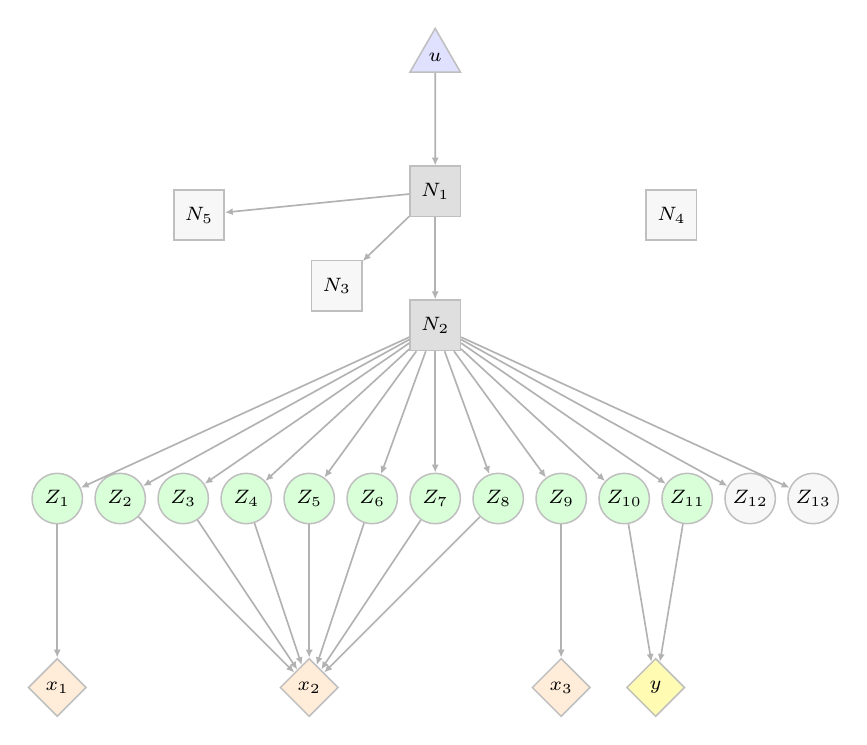
\begin{tikzpicture}[
    font=\small,
    vbase/.style   = {draw=gray!50, line width=0.55pt, inner sep=1pt,
                      font=\scriptsize},
    vinput/.style  = {vbase, regular polygon, regular polygon sides=3,
                      fill=blue!12, minimum size=7.4mm,
                      inner sep=-1pt},
    vnode/.style   = {vbase, rectangle, fill=gray!25, minimum size=6.4mm},
    vpruned/.style = {vbase, rectangle, fill=gray!6, minimum size=6.4mm},
    vlatent/.style = {vbase, circle, fill=green!15, minimum size=6.4mm},
    vunused/.style = {vbase, circle, fill=gray!6, minimum size=6.4mm},
    vobs/.style    = {vbase, diamond, fill=orange!15, minimum size=7.4mm},
    voutcome/.style= {vbase, diamond, fill=yellow!30, minimum size=7.4mm},
    arr/.style     = {-{Latex[length=1.0mm,width=0.9mm]}, semithick,
                      draw=gray!60},
  ]

  \node[vinput] (u) at (0.000cm, 0.000cm) {$ u $};
  \node[vnode] (N1) at (0.000cm, -1.700cm) {$ N_{1} $};
  \node[vnode] (N2) at (0.000cm, -3.400cm) {$ N_{2} $};
  \node[vpruned] (N3) at (-1.250cm, -2.900cm) {$ N_{3} $};
  \node[vpruned] (N5) at (-3.000cm, -2.000cm) {$ N_{5} $};
  \node[vpruned] (N4) at (3.000cm, -2.000cm) {$ N_{4} $};
  \node[vlatent] (Z1) at (-4.800cm, -5.600cm) {$ Z_{1} $};
  \node[vlatent] (Z2) at (-4.000cm, -5.600cm) {$ Z_{2} $};
  \node[vlatent] (Z3) at (-3.200cm, -5.600cm) {$ Z_{3} $};
  \node[vlatent] (Z4) at (-2.400cm, -5.600cm) {$ Z_{4} $};
  \node[vlatent] (Z5) at (-1.600cm, -5.600cm) {$ Z_{5} $};
  \node[vlatent] (Z6) at (-0.800cm, -5.600cm) {$ Z_{6} $};
  \node[vlatent] (Z7) at (0.000cm, -5.600cm) {$ Z_{7} $};
  \node[vlatent] (Z8) at (0.800cm, -5.600cm) {$ Z_{8} $};
  \node[vlatent] (Z9) at (1.600cm, -5.600cm) {$ Z_{9} $};
  \node[vlatent] (Z10) at (2.400cm, -5.600cm) {$ Z_{10} $};
  \node[vlatent] (Z11) at (3.200cm, -5.600cm) {$ Z_{11} $};
  \node[vunused] (Z12) at (4.000cm, -5.600cm) {$ Z_{12} $};
  \node[vunused] (Z13) at (4.800cm, -5.600cm) {$ Z_{13} $};
  \node[vobs] (x1) at (-4.800cm, -8.000cm) {$ x_{1} $};
  \node[vobs] (x2) at (-1.600cm, -8.000cm) {$ x_{2} $};
  \node[vobs] (x3) at (1.600cm, -8.000cm) {$ x_{3} $};
  \node[voutcome] (y) at (2.800cm, -8.000cm) {$ y $};

  \draw[arr] (u) -- (N1);
  \draw[arr] (N1) -- (N2);
  \draw[arr] (N1) -- (N3);
  \draw[arr] (N1) -- (N5);
  \draw[arr] (N2) -- (Z1);
  \draw[arr] (N2) -- (Z2);
  \draw[arr] (N2) -- (Z3);
  \draw[arr] (N2) -- (Z4);
  \draw[arr] (N2) -- (Z5);
  \draw[arr] (N2) -- (Z6);
  \draw[arr] (N2) -- (Z7);
  \draw[arr] (N2) -- (Z8);
  \draw[arr] (N2) -- (Z9);
  \draw[arr] (N2) -- (Z10);
  \draw[arr] (N2) -- (Z11);
  \draw[arr] (N2) -- (Z12);
  \draw[arr] (N2) -- (Z13);
  \draw[arr] (Z1) -- (x1);
  \draw[arr] (Z2) -- (x2);
  \draw[arr] (Z3) -- (x2);
  \draw[arr] (Z4) -- (x2);
  \draw[arr] (Z5) -- (x2);
  \draw[arr] (Z6) -- (x2);
  \draw[arr] (Z7) -- (x2);
  \draw[arr] (Z8) -- (x2);
  \draw[arr] (Z9) -- (x3);
  \draw[arr] (Z10) -- (y);
  \draw[arr] (Z11) -- (y);

\end{tikzpicture}
\end{document}
